%%%%%%%%%%%%%%%%%%%%%%%%%%%%%%%%%% Niels %%%%%%%%%%%%%%%%%%%%%%%%%%%%%
%%%%%%%%%%%%%%%%%
\section{State Space}

%---------------------------------------------------------------------------------
\subsection{Motivation}%----------------------------------------------------------
%---------------------------------------------------------------------------------

\begin{frame}{State Space}{Motivation}	
  \begin{itemize}
  	\item Angular velocity of the wheel using root locus design
  \end{itemize}
  \vspace{.5cm}
  \begin{minipage}{\linewidth}
  	\begin{minipage}{0.4\linewidth}
  		\begin{figure}
  			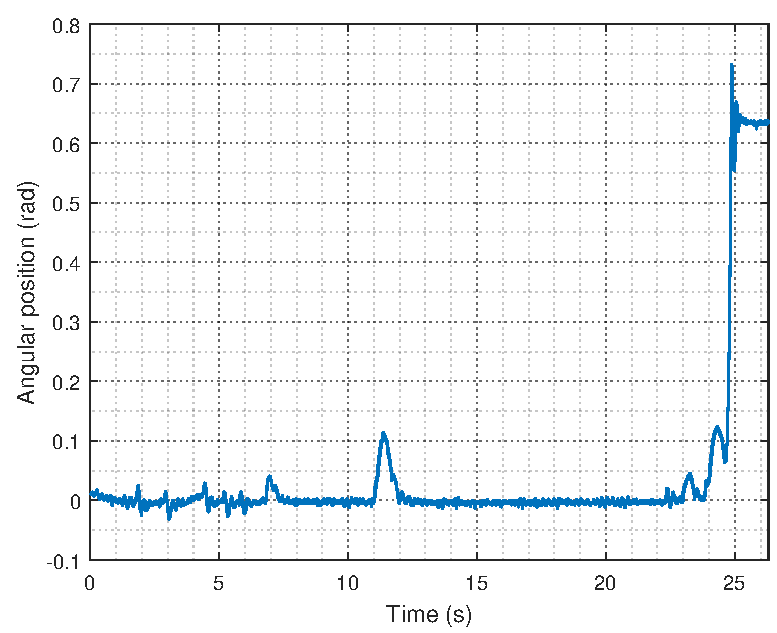
\includegraphics[scale=.35]{Pictures/positionRLTest}
  			\centering
  		\end{figure}
  	\end{minipage}
  	\hspace{0.1\linewidth}
  	\begin{minipage}{0.45\linewidth}
  		\begin{figure}[H]
  			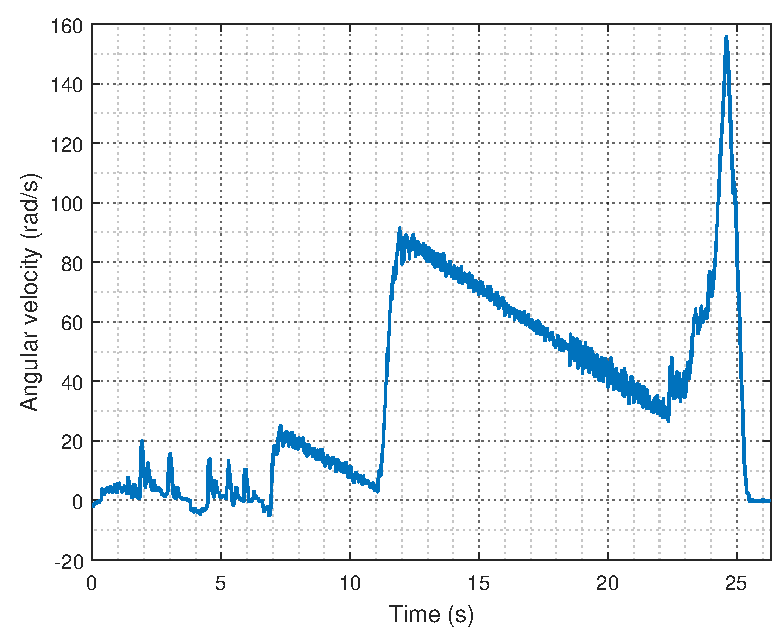
\includegraphics[scale=.35]{Pictures/wheelRLTest}
  			\centering
  		\end{figure}
  	\end{minipage}
  \end{minipage}
\end{frame}

\begin{frame}{State Space}{Motivation}
  \begin{itemize}
    \item Control of velocity for improved performance
    \item Classical cascade control is not feasible
  \end{itemize}
  \vspace{.2cm}
  \begin{figure}[H]
    \centering
      \begin{tikzpicture}[ auto,
                       thick,                         %<--setting line style
                       node distance=1.5cm,             %<--setting default node distance
                       scale=0.45,                     %<--|these two scale the whole thing
                       every node/.style={scale=0.50}, %<  |(always change both)
                       >/.tip={Triangle[angle=40:5pt]}
                       ]

    %-- Blocks creation --%
    \draw
      % DIRECT TERM %
      node[shape=coordinate][](input1) at (0,0){}
      node[shape=coordinate][](feedForward) at (0.5,0){}
      node(sum1) at (7.75,0) [sum] {\si{\sum}}
      node(sum2) at (9.25,0) [sum]{\si{\sum}}
      node(sum3) at (10.75,0) [sum]{\si{\sum}}

      node(torque2rotacc1) at (12.85,0) [block]{\large \si{\frac{1}{J_F + m_w \cdot {l_w}^{2}}}}

      node(integration1) at (15.75,0) [block] {\large \si{\frac{1}{s}}}
      node(integration2) at (18.2,0) [block] {\large \si{\frac{1}{s}}}

      node[shape=coordinate][](output) at (19,0){}
      node[shape=coordinate][](veloFeedbackNode) at (16.8,0){}
      node[shape=coordinate][](accFeedbackNode) at (14.5,0){}
    ;
    \draw
      % REACTION WHEEL EQUATIONS %  
      node(sum4) at (1.5,-1.6) [sum]{\si{\sum}}
      node(sum5) at (2.85,-1.6) [sum]{\si{\sum}}

      node(torque2rotacc2) at (4.3,-1.6) [block]{\large \si{\frac{1}{J_w \cdot s}}}
      % node(integration3) [block, right of = torque2rotacc2] {$\frac{1}{s}$}
      node(frictionWheel) at (6.9,-1.6) [block] {\large $B_w$}

      node[shape=coordinate][](veloWheelFeedback) at (7.75,-3.2){}
    ;
    \draw
      % FEEDBACKS %
      node(accFeedback) at (8, -4.8) [block] {\large \si{J_w}}
      node(veloFeedback) at (12.65,-1.6) [block] {\large \si{B_F}}
      node(angleFeedback) at (11.65,-3.2) [block] {\large \si{(m_F \cdot l_F + m_w \cdot l_w)g}}
    ;
    %-- Block linking --%
    % INPUT %
    \draw[-](input1)        -- node{\large \si{\tau_m(s)}}(feedForward);
    \draw[->](feedForward)  -- (sum1);

    % OUTPUT %
    \draw[-](integration2)  -- (output);
    \draw[->](output)       -- node {\large \si{\theta_{F}(s)}} (20,0);

    % DIRECT TERM %
    \draw[->] (sum1)            -- (sum2);
    \draw[->] (sum2)            -- (sum3);
    \draw[->] (sum3)            -- (torque2rotacc1);
    \draw[->] (torque2rotacc1)  -- node{\large \si{\ddot{\theta}_F(s)}}(integration1);
    \draw[->] (integration1)    -- node{\large \si{\dot{\theta}_F(s)}}(integration2);

    % REACTION WHEEL EQUATIONS %
    \draw[->] (feedForward)     |- (sum4);
    \draw[->] (sum4)            -- (sum5);
    \draw[->] (sum5)            -- (torque2rotacc2);
    \draw[->] (torque2rotacc2)  -- node{\large \si{\dot{\theta}_w(s)}}(frictionWheel);
    % \draw[->] (integration3)    -- (frictionWheel);
    \draw[->] (frictionWheel)   -| (sum1);

    \draw[-] (frictionWheel)       -| (veloWheelFeedback);
    \draw[->] (veloWheelFeedback)  -| (sum5);

    % FEEDBACKS
    \draw[->] (accFeedbackNode)  |- (accFeedback);
    \draw[->] (accFeedback)      -| (sum4);

    \draw[->] (output)           |- (angleFeedback);
    \draw[->] (angleFeedback)    -| (sum2);

    \draw[->] (veloFeedbackNode) |- (veloFeedback);
    \draw[->] (veloFeedback)     -| (sum3);

    %-- Nodes --%
    \draw%--------------------------------------------------------------
%      node at (input1)            [shift={(-0.04, -0.05 )}] {\Large \textopenbullet}
      node at (output)            [shift={( 0.007, -0.05 )}] {\Large \textbullet}
      node at (veloFeedbackNode)  [shift={( 0.007, -0.05 )}] {\Large \textbullet}
      node at (accFeedbackNode)   [shift={( 0.007, -0.05 )}] {\Large \textbullet}
      node at (feedForward)       [shift={( 0.007, -0.05 )}] {\Large \textbullet}
      node at (frictionWheel)     [shift={( 0.85, -0.04 )}] {\Large \textbullet}
    ;

    %-- Summation signs --%
      \draw%--------------------------------------------------------------
      node at (sum1) [right = -6.6mm, below = .6mm] {$-$}
      node at (sum1) [right = -3mm, below = 3.9mm]  {$+$} 
      node at (sum2) [right = -6.6mm, below = .6mm] {$+$}
      node at (sum2) [right = -3mm, below = 3.9mm]  {$+$}
      node at (sum3) [right = -6.6mm, below = .6mm] {$+$}
      node at (sum3) [right = -3mm, below = 3.9mm]  {$-$}
      node at (sum4) [right = -6.6mm, below = .6mm] {$+$}
      node at (sum4) [right = -3mm, below = 3.9mm]  {$-$}
      node at (sum5) [right = -6.6mm, below = .6mm] {$+$}
      node at (sum5) [right = -3mm, below = 3.9mm]  {$-$}
    ;

  \end{tikzpicture}
  \end{figure}
\end{frame}

%---------------------------------------------------------------------------------
\subsection{Model}%---------------------------------------------------------------
%---------------------------------------------------------------------------------

\begin{frame}{State Space}{Model}

  \begin{itemize}
  	\item State, output and input variables
  \end{itemize}

  \begin{minipage}{0.29\linewidth}
       	\begin{flalign}
       		\vec{x} = 
       		\begin{bmatrix}
       			\theta_F \\
       			\dot{\theta}_F \\ 
       			\dot{\theta}_w \\
       		\end{bmatrix}\nonumber
       	\end{flalign}  
      \end{minipage}
      %\hspace{0.03\linewidth}
      \begin{minipage}{0.29\linewidth}
       	\begin{flalign}
       		\vec{y} = 
       		\begin{bmatrix}
       			\theta_F \\
       			\dot{\theta}_w \\
       		\end{bmatrix}\nonumber
       	\end{flalign}
      \end{minipage}
      %\hspace{0.03\linewidth}
      \begin{minipage}{0.29\linewidth}
       	\begin{flalign}
       		\vec{u}= 
       		\begin{bmatrix}
       			\tau_m\\
       		\end{bmatrix}	\nonumber
       	\end{flalign}
    \end{minipage}
  \vspace{.5cm}
  \begin{itemize}
  	\item System of differential equations
  \end{itemize}
  %
  \begin{flalign}
  	&\hspace{.85cm} \si{\vec{\dot{x}} = f(\vec{x},\vec{u})}& \nonumber \\
  	&\hspace{.85cm} \si{\vec{y} = g(\vec{x},\vec{u})}& \nonumber
  \end{flalign}
\end{frame}

\begin{frame}{State Space}{Model}

  \only<1>
  {
    \tikz[overlay,xshift=4.5em,yshift=7ex]{\draw node {
      \begin{minipage}{0.01\linewidth}
      	  \begin{flalign}
        	  	& \hspace{1 cm} \si{\vec{\dot{x}}(t) =\ } \si{ \vec{A} \cdot \vec{x}(t) + \vec{B} \cdot \vec{u}(t)} \nonumber \\
        	  	& \hspace{1 cm} \si{\vec{y}(t) =\ } \si{ \vec{C} \cdot \vec{x}(t) } \nonumber
      	  \end{flalign}
      \end{minipage}
      \begin{minipage}{0.01\linewidth}
        \begin{tabular}{ p{.1cm} l l l}
          &&\\
          	& \si{\vec{A}=\frac{\partial}{\partial \vec{x}} \ f(\vec{x_o},\vec{u_o})}			& state     \\                       
          	& \si{\vec{B}=\frac{\partial}{\partial \vec{u}} \ f(\vec{x_o},\vec{u_o})}			& input     \\ 
          	& \si{\vec{C}=\frac{\partial}{\partial \vec{x}} \ g(\vec{x_o},\vec{u_o})}			& output
        \end{tabular} 
      \end{minipage}
    };}
  }
  
  \only<2>
  {  
    \tikz[overlay,xshift=9.5em,yshift=13ex]{\draw node [fontscale=\footnotesize]{
                \si{\ddot{\theta}_F = -\frac{B_F}{J_F + m_w \cdot {l_w}^2} \cdot \dot{\theta}_F + \frac{(m_F \cdot l_F + m_w \cdot l_w) \cdot g}{J_F + m_w \cdot {l_w}^2} \cdot \theta_F}
                };}
    \tikz[overlay,xshift=9.5em,yshift=9.3ex]{\draw node [fontscale=\footnotesize]{
                 \si{- \frac{1}{J_F + m_w \cdot {l_w}^2} \cdot \tau_m + \frac{B_w}{J_F + m_w \cdot {l_w}^2} \cdot \dot{\theta}_w}
                 };}
    \tikz[overlay,xshift=10.2em,yshift=4ex]{\draw node [fontscale=\footnotesize]{
                  \si{\ddot{\theta}_w = \frac{J_w+J_F+m_w \cdot {l_w}^{2}}{J_w \cdot (J_F+m_w \cdot {l_w}^{2})} \cdot \tau_m - \frac{(J_w+J_F+{l_w}^{2} \cdot m_w) \cdot B_w}{J_w \cdot (J_F+m_w \cdot  {l_w}^2)} \cdot \dot{\theta}_w}
                };}
    \tikz[overlay,xshift=9.7em,yshift=0ex]{\draw node [fontscale=\footnotesize]{
                  \si{- \frac{(m_F \cdot l_F + m_w \cdot l_w) \cdot g}{J_F+m_w \cdot {l_w}^{2}} \cdot \theta_F + \frac{B_F}{J_F+m_w \cdot {l_w}^{2}} \cdot \dot{\theta}_F}
             };} 
  }
  
  \only<1-2>
  {
    \tikz[overlay,xshift=11.5em,yshift=-7ex]{\draw node {
        \begin{tikzpicture}[ auto,
                       thick,                         %<--setting line style
                       node distance=1.5cm,             %<--setting default node distance
                       scale=.9,                     %<--|these two scale the whole thing
                       every node/.style={scale=.9}, %<  |(always change both)
                       >=triangle 45 ]                %<--sets the arrowtype
    
    \draw%-----------------------------------------------------------------------------------------
    	%Drawing Input/Output:
    	node[shape=coordinate][](input1) at (0,0){}
    	node[shape=coordinate][](output1) at (8,0){}
     	%Drawing the Equation Blocks:   	
      	node(A) at (4.5,-1.5) [block] {A} 
     	node(B) at (1.5,0) [block] {B}
     	node(C) at (6.5,0) [block] {C}
%      	node(D) at (4.5,1.5) [block] {D}  
	    node(int) at (4.5,0) [block] {\si{\int}}  
    	%Drawing the Sumation Blocks:	    	 	
    	node(sum1) [sum, right of = B] {\si{\sum}}
%    	node(sum2) [sum, right of = C] {\si{\sum}}
    	%Drawing the Feedback/Feedforward Nodes:    	
    	node[shape=coordinate][](FeedforwardNode) at (0.75,0){}
    	node[shape=coordinate][](FeedbackNode) at (5.5,0){}  	
    	     
    ;%---------------------------------------------------------------------------------------------
   
    %Joining the Blocks
  	\draw[->](input1) -- node {u}(B);
  	\draw[->](B) -- node {}(sum1);
  	\draw[->](sum1) -- node {\si{\dot x}}(int);  	
  	\draw[->](int) -- node {x}(C);
  	\draw[->](C) -- node {y}(output1);
  	
%  	\draw[->](FeedforwardNode) |- node{} (D);
%  	\draw[->](D) -| node{} (sum2);

  	\draw[-] (FeedbackNode) |- (A);
  	\draw[->] (A)   -| (sum1);

    %Drawing node(s) with \textbullet
    \draw%--------------------------------------------------------------
%      node at (input1)  [shift={(-0.04, -0.04 )}] {\large \textbullet}
    	% node at (output1) [shift={( 0.008, -0.02 )}] {\textbullet}
    ;%------------------------------------------------------------------
  \end{tikzpicture}
    };}
    \tikz[overlay,xshift=7.5em,yshift=-16ex]{\draw node {
        \begin{minipage}{0.01\linewidth}
         	\begin{flalign}
         		\vec{x} = 
         		\begin{bmatrix}
         			\theta_F \\
         			\dot{\theta}_F \\ 
         			\dot{\theta}_w \\
         		\end{bmatrix}	\textbf{,}\ \nonumber
         	\end{flalign}  
        \end{minipage}
        %\hspace{0.03\linewidth}
        \begin{minipage}{0.01\linewidth}
         	\begin{flalign}
         		\vec{y} = 
         		\begin{bmatrix}
         			\theta_F \\
         			\dot{\theta}_w \\
         		\end{bmatrix}	\textbf{,}\ \nonumber
         	\end{flalign}
        \end{minipage}
        %\hspace{0.03\linewidth}
        \begin{minipage}{0.01\linewidth}
         	\begin{flalign}
         		\vec{u}= 
         		\begin{bmatrix}
         			\tau_m\\
         		\end{bmatrix}	\nonumber
         	\end{flalign}
      \end{minipage}
    };}
  }   
\end{frame}

%---------------------------------------------------------------------------------
\subsection{Controller Design}%---------------------------------------------------
%---------------------------------------------------------------------------------
\begin{frame}{State Space}{Controller Design}
  \begin{itemize}
    \item Eigenvalues of \si{A - BK}
    \item Pole placement
  \end{itemize}

  \begin{displaymath}
  	\hspace{-5cm}\si{\vec{\dot{x}}(\vec{t}) = (\vec{A}-\vec{B}\vec{K}) \cdot \vec{x}(\vec{t})} \nonumber
  \end{displaymath}
  
  \begin{figure}[H]
      \centering
      \begin{tikzpicture}[ auto,
					thick,                         %<--setting line style
					node distance=1.5cm,             %<--setting default node distance
					scale=1,                     %<--|these two scale the whole thing
					every node/.style={scale=1}, %<  |(always change both)
					>=triangle 45 ]                %<--sets the arrowtype

	\draw%-----------------------------------------------------------------------------------------
	%Drawing Input/Output:
	node[shape=coordinate][](input1) at (0,0){}
	node[shape=coordinate][](inputFeedback) at (.3,0){}
	node[shape=coordinate][](output1) at (8,0){}
	%Drawing the Equation Blocks:   	
	node(A) at (4,-1.5) [block] {A} 
	node(B) at (1.5,0) [block] {B}
	node(C) at (6.5,0) [block] {C}
	node(int) at (4.5,0) [block] {\si{\int}} 
	node(K) at (2.8,-2.5) [block] {-K}	
	%Drawing the Sumation Blocks:	    	 	
	node(sum1) [sum, right of = B] {\si{\sum}}
	%Drawing the Feedback/Feedforward Nodes:    	
	node[shape=coordinate][](FeedbackNode) at (5.2,0){}  	
	node[shape=coordinate][](FeedbackNode2) at (5.6,0){} 
	
	;%---------------------------------------------------------------------------------------------

	%Joining the Blocks
	\draw[->](input1) -- node {u}(B);
	\draw[->](B) -- node {}(sum1);
	\draw[->](sum1) -- node {\si{\dot x}}(int);  	
	\draw[->](int) -- node {x}(C);
	\draw[->](C) -- node {y}(output1);

	\draw[->] (FeedbackNode) |- (A);
	\draw[->] (A)   -| (sum1);
	
	\draw[->] (FeedbackNode2) |- (K);
	\draw[-] (K)   -| (inputFeedback);

	%Drawing node(s) with \textbullet
	\draw%--------------------------------------------------------------
%	node at (input1)  [shift={(-0.08, -0.02 )}] {\large \textbullet}
	% node at (output1) [shift={( 0.008, -0.04 )}] {\textbullet}
	;%------------------------------------------------------------------

\end{tikzpicture}
  \end{figure}
\end{frame}

\begin{frame}{State Space}{Controller Design}
  \begin{itemize}
    \item Controller reacting to disturbance
    \item Different pole placements
    \item The yellow was chosen
  \end{itemize}
  \vspace{.5cm}
  \hspace{0.03\linewidth}
  \begin{minipage}{\linewidth}
   	\begin{minipage}{0.45\linewidth}
   		\begin{figure}[H]
   			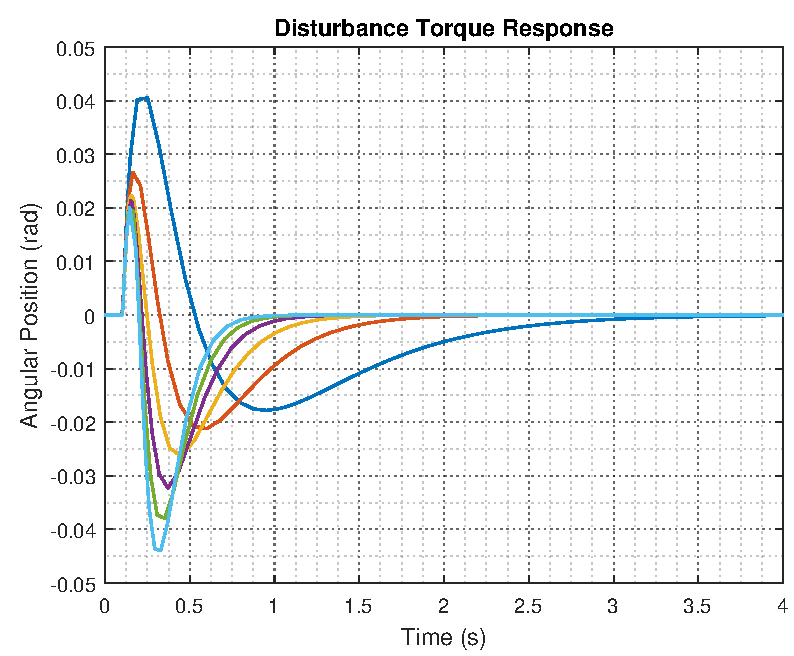
\includegraphics[scale=.35]{Pictures/disturbanceStateSpace}
   			\centering
   		\end{figure}
   	\end{minipage}
   	\hspace{0.03\linewidth}
   	\begin{minipage}{0.45\linewidth}
   		\begin{figure}[H]
   			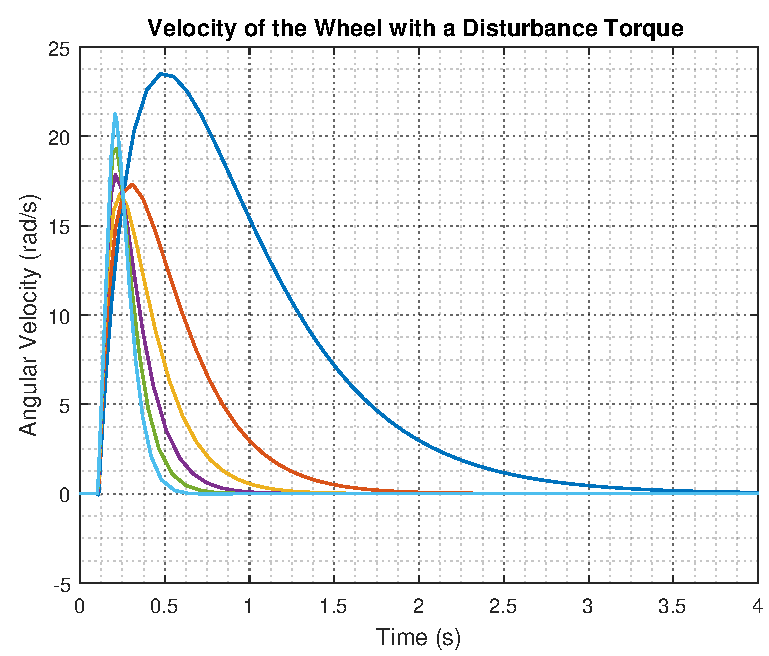
\includegraphics[scale=.35]{Pictures/disturbanceStateSpaceWheel}
   			\centering
   		\end{figure}
   	\end{minipage}
  \end{minipage}
\end{frame}

%---------------------------------------------------------------------------------
\subsection{Controller Analysis}%-------------------------------------------------
%---------------------------------------------------------------------------------

\begin{frame}{State Space}{Controller Analysis}
    \begin{minipage}{\linewidth}
    	\begin{minipage}{0.4\linewidth}
    		\begin{figure}
    			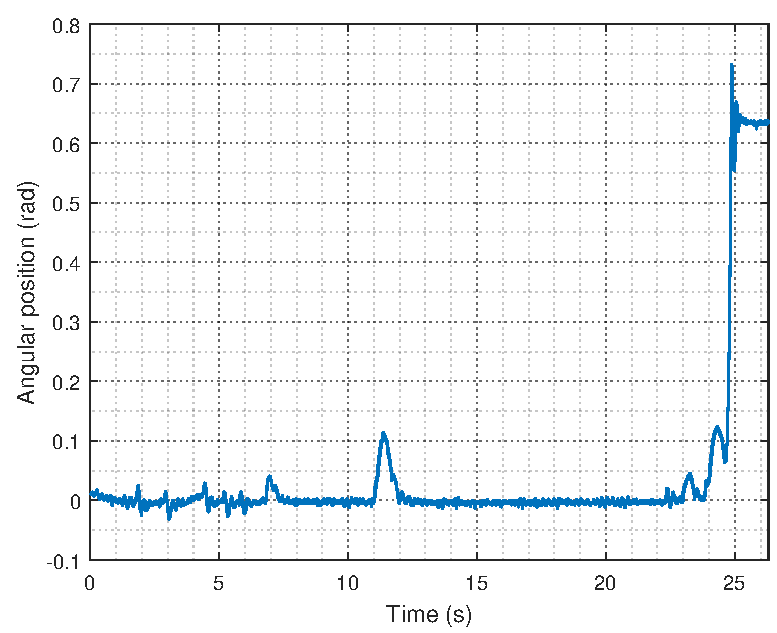
\includegraphics[scale=.35]{Pictures/positionRLTest}
    			\centering
    		\end{figure}
    	\end{minipage}
    	\hspace{0.1\linewidth}
    	\begin{minipage}{0.45\linewidth}
    		\begin{figure}[H]
    			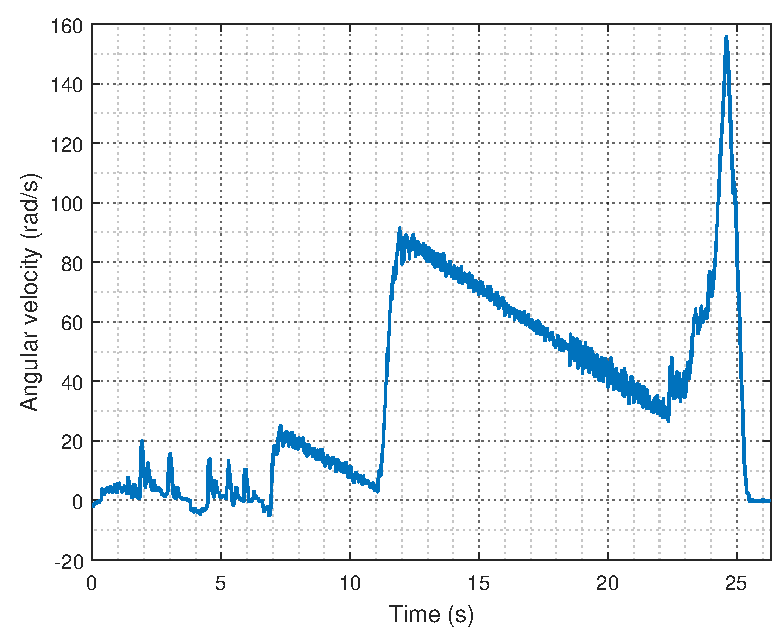
\includegraphics[scale=.35]{Pictures/wheelRLTest}
    			\centering
    		\end{figure}
    	\end{minipage}
    \end{minipage}
  \vspace{.5cm}
  \begin{minipage}{\linewidth}
   	\begin{minipage}{0.45\linewidth}
   		\begin{figure}[H]
   			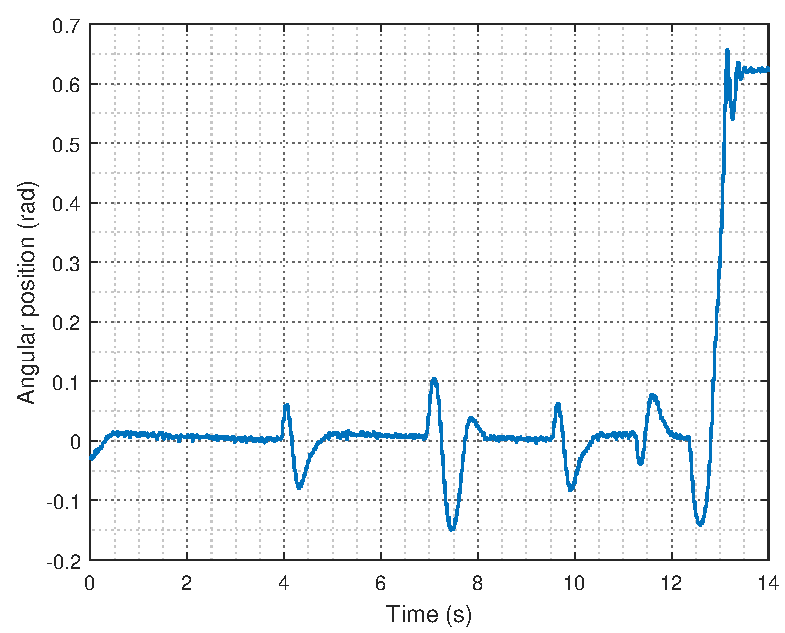
\includegraphics[scale=.35]{Pictures/positionSSTest}
   			\centering
   		\end{figure}
   	\end{minipage}
   	\hspace{0.03\linewidth}
   	\begin{minipage}{0.45\linewidth}
   		\begin{figure}[H]
   			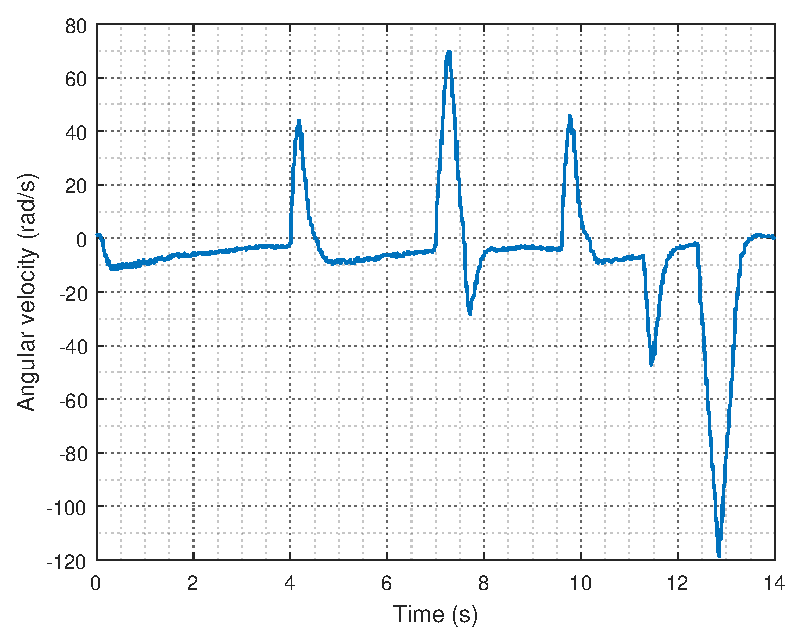
\includegraphics[scale=.35]{Pictures/wheelSSTest}
   			\centering
   		\end{figure}
   	\end{minipage}
  \end{minipage}
\end{frame}


% %---------------------------------------------------------------------------------
% \subsection{Animation Test}%------------------------------------------------------
% %---------------------------------------------------------------------------------

% \begin{frame}{Animation Test}{wooohooo}
%   \transduration<0-19>{1.5}
%   \multiinclude[format=png, graphics={width=\textwidth}]{Pictures/optJoinedFit/cost}
%   %\animategraphics[autoplay,loop,width=\linewidth]{1}{Pictures/cost-}{0}{19}
% \end{frame}